\chapter[Fundamentação Teórica]{Fundamentação Teórica}

O estudo de Inteligência Artificial vem sendo cada vez mais comum na comunidade de tecnologia da informação para a criação de sistemas que buscam automatizar e auxiliar de maneira mais eficiente o trabalho humano. O ramo de aplicação para essa tecnologia é imensa, e o uso para a área do Direito não seria diferente.

\section{Aprendizagem de Máquina}

Aprendizado de Máquina do inglês \textit{Machine Learning} (ML) é uma das subáreas da Inteligência Artificial que visa criar mecanismos que possibilitem fazer com que uma máquina possa "aprender" sobre um determinado problema a partir de um conjunto de dados de entrada. Em outras palavras, ML permite que um dado algoritmo desenvolva uma função matemática que consiga representar tal conjunto de dados. Com essa função ou modelo matemático, é possível agora realizar inferências sobre outros dados, desde que esses sejam relacionados à mesma problemática \cite{deep-learning-book}.

O processo de aprendizagem se da início a partir de observações ou dados, como exemplos, experiência direta ou instruções que possibilitem identificar padrões do dado para realizar e atingir melhores decisões em futuras apresentações ou exemplos de dados que possam ser fornecidas. Dentro do processo de permitir que uma máquina aprenda, existem três áreas as quais os mecanismos de aprendizagem são classificados \cite{python-ml}:

\begin{itemize}
  \item \textbf{Aprendizado supervisionado:} o objetivo principal de algoritmos supervisionados é conseguir desenvolver um modelo matemático a partir de um conjunto de dados anotados, no caso, dados de treinamento. O \textit{supervisionado} diz respeito ao conjunto de dados os quais já se sabe a saída esperada, ou seja, o dado já é anotado previamente. Em geral, esses algoritmos são utilizados para problemas de classificação e regressão.
  \begin{figure}
    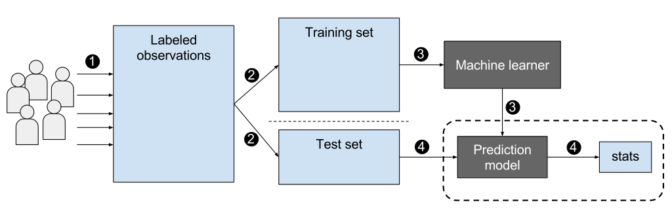
\includegraphics[width=\linewidth]{figuras/nvidia-supervised-learning.png}
    \caption{Aprendizado supervisionado \color{red} OBS: COLOCAR FONTE}
    \label{fig:nvidia-supervised-learning}
  \end{figure}
  \newpage
  \item \textbf{Aprendizado não supervisionado:} diz respeito aos métodos de aprendizagem de máquina os quais utiliza-se como dado de entrada um dado que não possui nenhum tipo de anotação e que, muitas vezes, sua estrutura é desconhecida.

  Tal processo de aprendizagem permite extrair características relevantes sobre o dado que possam servir de insumo para uma futura categorização e classificação do mesmo. Dependendo do problema em questão, a aprendizagem supervisionada pode organizar o dado em diferentes categorias \cite{learning-types} como clusterização, associação, \textit{autoencoders}, \textit{anomaly detection}, etc.

  \item \textbf{Aprendizado semi-supervisionado:} já o aprendizado semi-supervisionado junta um pouco dos dois mundos: dados com registros anotados e também dados com registros não anotados. A aplicabilidade para esse tipo de aprendizagem é quando se possui um dado onde não é trivial extrair informações relevantes sobre ele e tampouco é realizar toda a anotação da amostra em questão \cite{learning-types}.
\end{itemize}

Dentro dos tipos de algoritmos que podem ser utilizados para construir ML, um que é bastante notado, mais comumente para algoritmos supervisionados 